\documentclass[models.tex]{subfiles} 
\begin{document}
\thispagestyle{empty}
\scalebox{3}{Model: SL-2042-79T}\\[1.4cm]
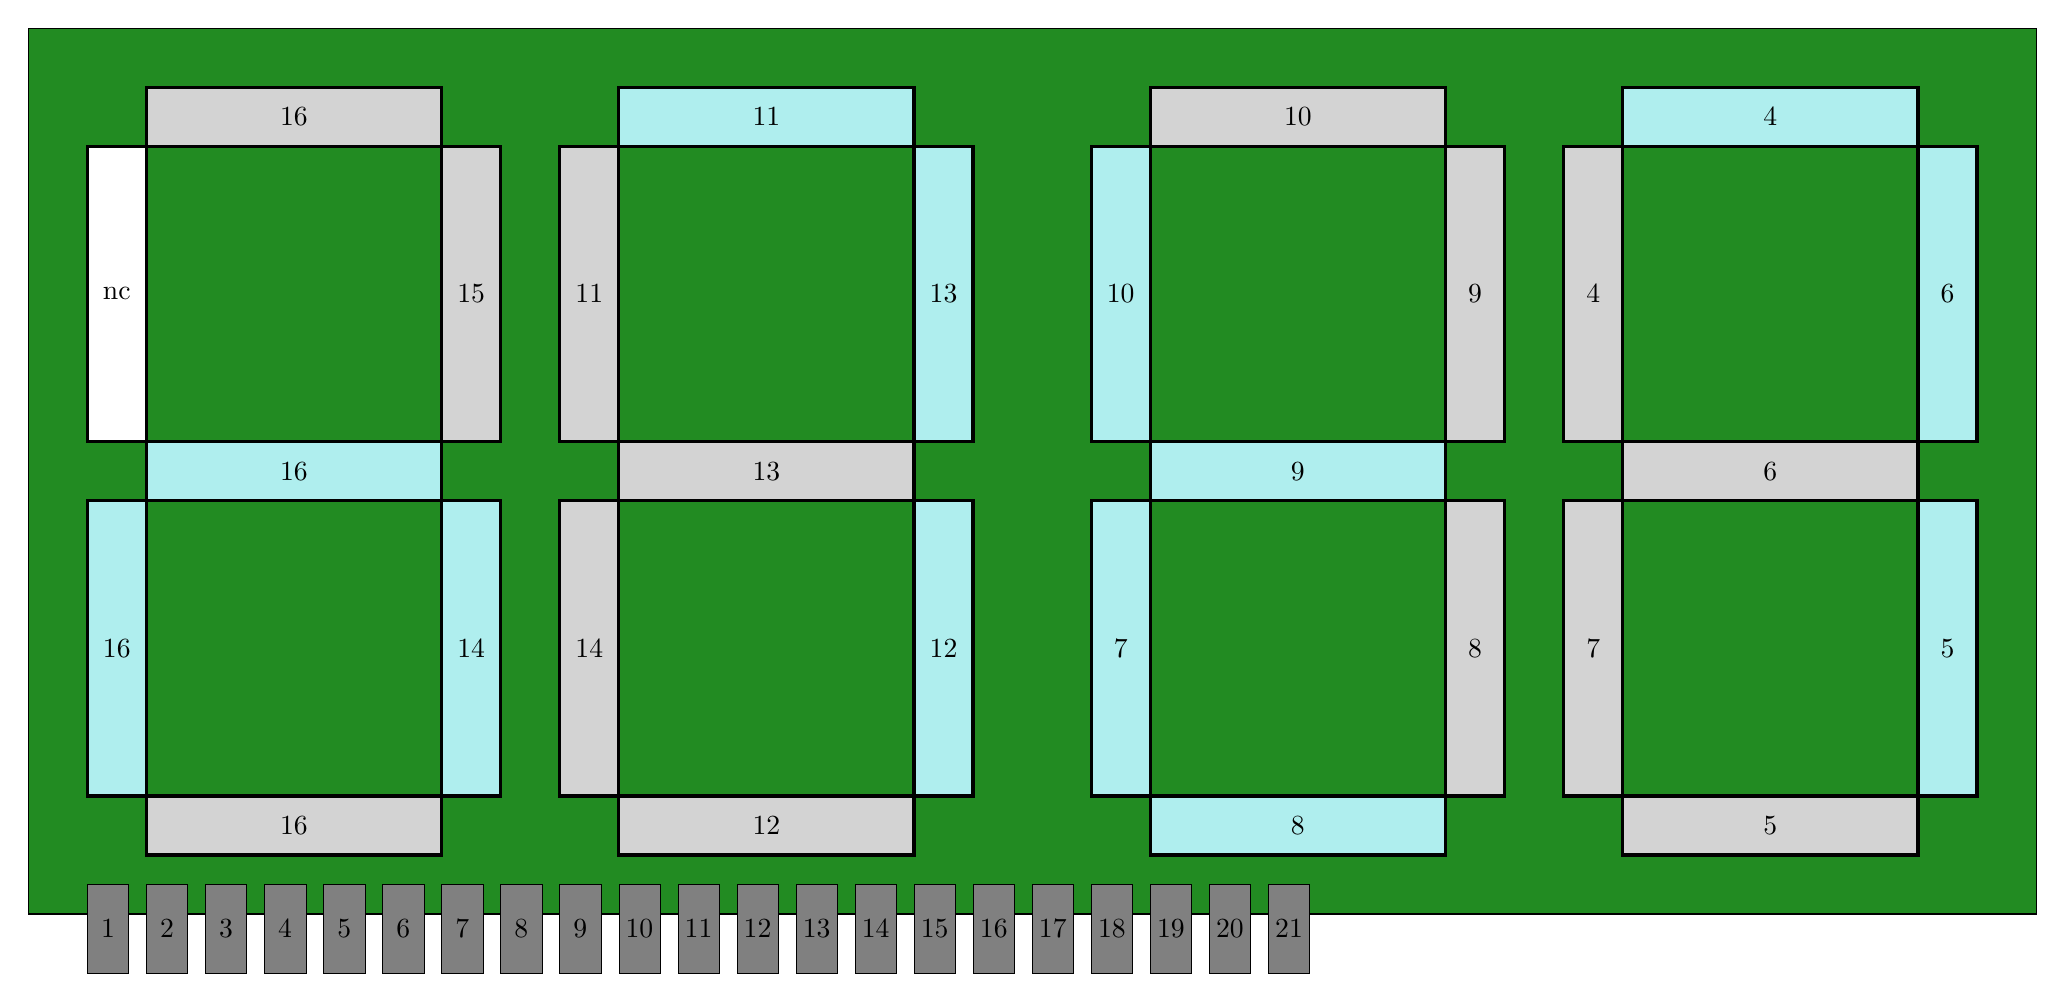
\begin{tikzpicture}[scale=0.75]
	%background
	\draw [fill=ForestGreen, thin] (-1, -1) rectangle (33, 14);
	
	%pinout
	\draw [fill=Gray, very thin] (0, -0.5) rectangle (0.7, -2) node[pos=0.5]{1};
	\draw [fill=Gray, very thin] (1, -0.5) rectangle (1.7, -2) node[pos=0.5]{2};
	\draw [fill=Gray, very thin] (2, -0.5) rectangle (2.7, -2) node[pos=0.5]{3};
	\draw [fill=Gray, very thin] (3, -0.5) rectangle (3.7, -2) node[pos=0.5]{4};
	\draw [fill=Gray, very thin] (4, -0.5) rectangle (4.7, -2) node[pos=0.5]{5};
	\draw [fill=Gray, very thin] (5, -0.5) rectangle (5.7, -2) node[pos=0.5]{6};
	\draw [fill=Gray, very thin] (6, -0.5) rectangle (6.7, -2) node[pos=0.5]{7};
	\draw [fill=Gray, very thin] (7, -0.5) rectangle (7.7, -2) node[pos=0.5]{8};
	\draw [fill=Gray, very thin] (8, -0.5) rectangle (8.7, -2) node[pos=0.5]{9};
	\draw [fill=Gray, very thin] (9, -0.5) rectangle (9.7, -2) node[pos=0.5]{10};
	\draw [fill=Gray, very thin] (10, -0.5) rectangle (10.7, -2) node[pos=0.5]{11};
	\draw [fill=Gray, very thin] (11, -0.5) rectangle (11.7, -2) node[pos=0.5]{12};
	\draw [fill=Gray, very thin] (12, -0.5) rectangle (12.7, -2) node[pos=0.5]{13};
	\draw [fill=Gray, very thin] (13, -0.5) rectangle (13.7, -2) node[pos=0.5]{14};
	\draw [fill=Gray, very thin] (14, -0.5) rectangle (14.7, -2) node[pos=0.5]{15};
	\draw [fill=Gray, very thin] (15, -0.5) rectangle (15.7, -2) node[pos=0.5]{16};
	\draw [fill=Gray, very thin] (16, -0.5) rectangle (16.7, -2) node[pos=0.5]{17};
	\draw [fill=Gray, very thin] (17, -0.5) rectangle (17.7, -2) node[pos=0.5]{18};
	\draw [fill=Gray, very thin] (18, -0.5) rectangle (18.7, -2) node[pos=0.5]{19};
	\draw [fill=Gray, very thin] (19, -0.5) rectangle (19.7, -2) node[pos=0.5]{20};
	\draw [fill=Gray, very thin] (20, -0.5) rectangle (20.7, -2) node[pos=0.5]{21};
	
	%1st digit
	\draw [fill=LightGray, very thick] (1, 13) rectangle (6, 12) node[pos=0.5]{16};
	\draw [fill=LightGray, very thick] (6, 12) rectangle (7, 7) node[pos=0.5]{15};
	\draw [fill=PaleTurquoise, very thick] (6, 6) rectangle (7, 1) node[pos=0.5]{14};
	\draw [fill=LightGray, very thick] (1, 0) rectangle (6, 1) node[pos=0.5]{16};
	\draw [fill=PaleTurquoise, very thick] (0, 1) rectangle (1, 6) node[pos=0.5]{16};
	\draw [fill=White, very thick] (0, 7) rectangle (1, 12) node[pos=0.5]{nc};
	\draw [fill=PaleTurquoise, very thick] (1, 6) rectangle (6, 7) node[pos=0.5]{16};
	%2nd digit
	\draw [fill=PaleTurquoise, very thick] (8+1, 13) rectangle (8+6, 12) node[pos=0.5]{11};
	\draw [fill=PaleTurquoise, very thick] (8+6, 12) rectangle (8+7, 7) node[pos=0.5]{13};
	\draw [fill=PaleTurquoise, very thick] (8+6, 6) rectangle (8+7, 1) node[pos=0.5]{12};
	\draw [fill=LightGray, very thick] (8+1, 0) rectangle (8+6, 1) node[pos=0.5]{12};
	\draw [fill=LightGray, very thick] (8+0, 1) rectangle (8+1, 6) node[pos=0.5]{14};
	\draw [fill=LightGray, very thick] (8+0, 7) rectangle (8+1, 12) node[pos=0.5]{11};
	\draw [fill=LightGray, very thick] (8+1, 6) rectangle (8+6, 7) node[pos=0.5]{13};
	%3rd digit
	\draw [fill=LightGray, very thick] (17+1, 13) rectangle (17+6, 12) node[pos=0.5]{10};
	\draw [fill=LightGray, very thick] (17+6, 12) rectangle (17+7, 7) node[pos=0.5]{9};
	\draw [fill=LightGray, very thick] (17+6, 6) rectangle (17+7, 1) node[pos=0.5]{8};
	\draw [fill=PaleTurquoise, very thick] (17+1, 0) rectangle (17+6, 1) node[pos=0.5]{8};
	\draw [fill=PaleTurquoise, very thick] (17+0, 1) rectangle (17+1, 6) node[pos=0.5]{7};
	\draw [fill=PaleTurquoise, very thick] (17+0, 7) rectangle (17+1, 12) node[pos=0.5]{10};
	\draw [fill=PaleTurquoise, very thick] (17+1, 6) rectangle (17+6, 7) node[pos=0.5]{9};
	%4th digit
	\draw [fill=PaleTurquoise, very thick] (25+1, 13) rectangle (25+6, 12) node[pos=0.5]{4};
	\draw [fill=PaleTurquoise, very thick] (25+6, 12) rectangle (25+7, 7) node[pos=0.5]{6};
	\draw [fill=PaleTurquoise, very thick] (25+6, 6) rectangle (25+7, 1) node[pos=0.5]{5};
	\draw [fill=LightGray, very thick] (25+1, 0) rectangle (25+6, 1) node[pos=0.5]{5};
	\draw [fill=LightGray, very thick] (25+0, 1) rectangle (25+1, 6) node[pos=0.5]{7};
	\draw [fill=LightGray, very thick] (25+0, 7) rectangle (25+1, 12) node[pos=0.5]{4};
	\draw [fill=LightGray, very thick] (25+1, 6) rectangle (25+6, 7) node[pos=0.5]{6};
\end{tikzpicture}

1: common cathode 1.

2: common cathode 2.
\end{document}